\section{Aufgabenstellung}
\label{sec:aufgabe}
Es soll ein Gerät entwickelt werden, das Bälle in einen Korb werfen kann. 
Dies soll autonom erfolgen. 
\begin{figure}[h!]
    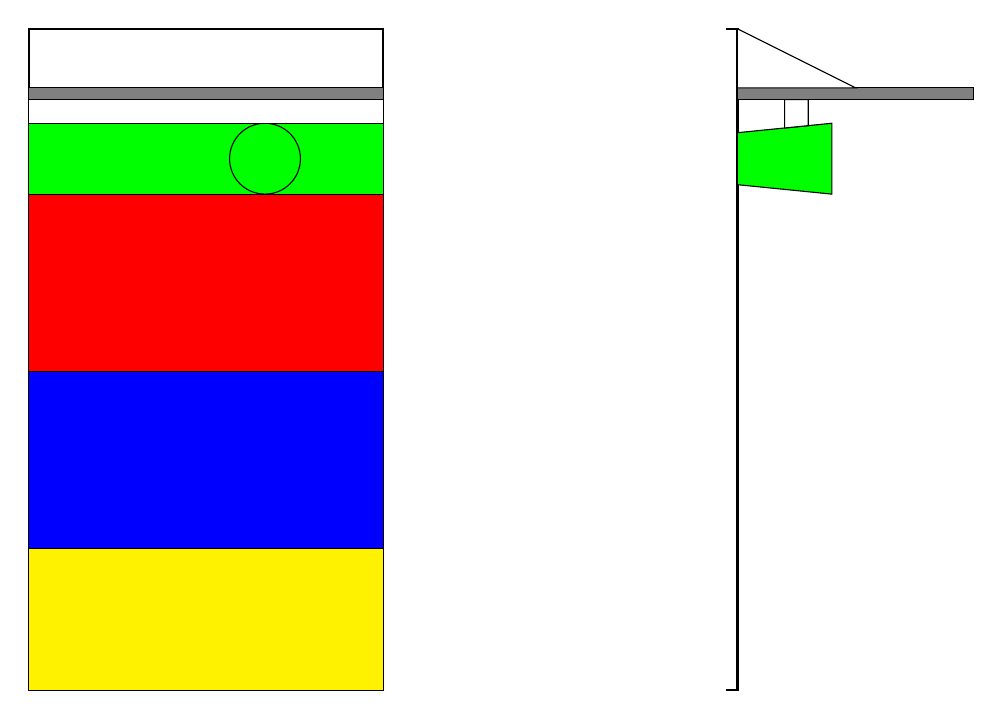
\begin{tikzpicture}[scale=0.03]
        % playfield frame
        \draw[thick] (0,0) rectangle (150,280);
        \draw[thick] (295,0) -- (300,0) -- (300,280) -- (295,280);
        % startfield
        \draw[fill=yellow] (0,0) rectangle (150,60);
        % move field
        \draw[fill=blue] (0,60) rectangle (150,135);
        % border line
        \draw[thick] (0,135) -- (150,135);
        % void field
        \draw[fill=red] (0,135) rectangle (150,210);
        % basket field
        \draw[fill=green] (0,210) rectangle (150,240);
        % basket
        \draw[fill=green] (100,225) circle [radius=15];
        \draw[fill=green] (300,214) -- (340,210) -- (340,240) -- (300,236) -- (300,214);
        % gap filler
        \draw[fill=white] (0,240) rectangle (150,250);
        \draw[fill=white] (320,250) -- (320,238) -- (330,239) -- (330,250) -- (320,250);
        % wall
        \draw[fill=gray] (0,250) rectangle (150,255);
        \draw[fill=gray] (300,250) rectangle (400,255);
        \draw[fill=white] (300,255) -- (350,255) -- (300,280) -- (300,255);
    \end{tikzpicture}
    \caption{Spielfeld}
    \label{fig:playfield}
\end{figure}

\subsection{Eigene Anforderungen}
